\documentclass{report}
\usepackage[utf8]{inputenc}
\usepackage{graphicx}
\graphicspath{ {./images/} }
\usepackage{multicol}

% width,height
\usepackage[a4paper, total={7in, 10in}]{geometry}

\title{IoT - Research Paper Summary}
\author{Smruthi Balaji}
\date{\today}

\begin{document}

    \begin{titlepage}
    \centering
        \vspace*{2cm}
        \Huge
        \textbf{Predicting Health of Fleet Equipment using IoT}
        
        \vspace*{0.6cm}
        \Large
        \textit{Research Paper Summary}
        
        \normalsize
        \vspace*{1.5cm}
        Smruthi Balaji\\
        \vspace{0.2cm}
        2101110125\\
        \vspace{0.2cm}
        AI-DS B\\
        
        \vfill
        
        %\large
        %32. Kandinsky Patterns
        
        %\begin{figure}[h]   % Figure Environment
        %    \centering
        %    \includegraphics[width = 2cm, scale=0.25]{logo2}  % including the picture
        %    \caption{Smruthi Balaji}
        %    \label{fig:my_image}
        %\end{figure}
        
        %\includegraphics[scale = 0.5]{MVP Architecture.png}
        
        \vfill
        
        %\includegraphics[scale=0.5]{logo}
        
        
\includegraphics{logo3}\\
        Computer Science and Engineering\\
        Shiv Nadar University, Chennai\\
        22 January 2022
        \vspace*{1cm}
    
\end{titlepage}

    
    \begin{center}
        \section*{Predicting Health of Fleet Equipment using IoT}
    \end{center}
\setlength{\columnsep}{1.0cm}
    \large
    \section*{Introduction}
    Internet of Things (IoT) is an up-and-coming technology that connects a vast network of devices to the internet so that they can sense and interact with their environment and the data collected can be analyzed. IoT is made up of five layers: sensing, network, storage, learning and application. Analysis of sensor data is done by the learning layer, during which anomalies can be detected. Predictive maintenance can help with preventing failures, unscheduled maintenance and downtime.\\
    
    Currently, there is a predictive maintenance system for a bus fleet called COSMO, a data-driven sensor selection strategy that focuses on less critical equipment. It runs experiments and select sensors based on entropy and stability. Anomalies are detected and the repair diagnosis is done using a vehicle service record database (VSRDB). However, the VSRDB isn't properly formatted so some repairs were made too early and they mention that their sensor selection method is not optimized. The author proposes an IoT architecture with three layers, which encompass the functions of the five layers mentioned previously, as well as a feature to improve sensor selection.\\  
    
    The perception layer performs sensing, lightweight storage, networking, and machine learning, i.e, it provides the interface to low-level nodes. This layer has a vehicle node (VN), which reads J1939 traffic to collect data and lightly analyze it. The middleware layer is does the same tasks as the perception layer but heavyweight. This layer contains the server leader node (SLN), which is found in the fog or the cloud and manages the VNs of a region. It also performs fleet-wide data analytics. The application layer is the same as in the current model. The root node (RN) is fleet system's access point and is responsible for interfacing IoT applications and connecting nodes to the system.\\
    
    ICOSMO is a method that attempts to improve the method of sensor selection using a semi-supervised machine learning approach. The method tries to reduce the occurrences of NFFs using a black box document retrieval algorithm (BBDRA).\\
        
        A minimally viable prototype (MVP) of this architecture has been implemented.
    
%\begin{multicols}{2}    
    \section*{Architecture}
    %our understanding of what the authors have contributed or raised as comments regarding the topic.  
    \begin{enumerate}
        \item \textbf{Perception Layer}  - Interacts with the fog (a layer of computing located between physical devices and the cloud) and the embedded systems. The task of the perception layer is to  sense , perform lightweight storage, networking and machine learning (to develop algorithms and to implement and accomplish tasks). \\																		It provides interface to the lower level nodes. The Vehicle Node (VN) is a part of this layer. It consists of a J1939 network and a gateway which helps read the J1939 traffic and acquire and analyze data from sensors. It stores the collected data using an embedded database.\\

        \item \textbf{Middleware Layer} - Acts as a bridge between the perception layer and the cloud and helps to store information from the perception layer. It performs more heavy duty tasks (networking, machine learning) compared to the perception layer which allows it to communicate with the perception layer nodes.  		\\																							Sever Leader Node (SLN) is a part of this layer. It is a type of a software that sits between operating system and other programs and is located in the fog or the cloud. The SLN is responsible for managing Virtual Networks in a particular area.     \\                                                                                                                       																																								
        \item \textbf{Application Layer} - It enables communication and interaction between different services. The Root Node (RN) is a part of this layer. It acts as a point of access for the fleet system and provides an interface for IoT applications. It has a server and agent installed which gives administrators the ability to change software on the nodes from outside the system.

    \end{enumerate}


    \begin{center}
    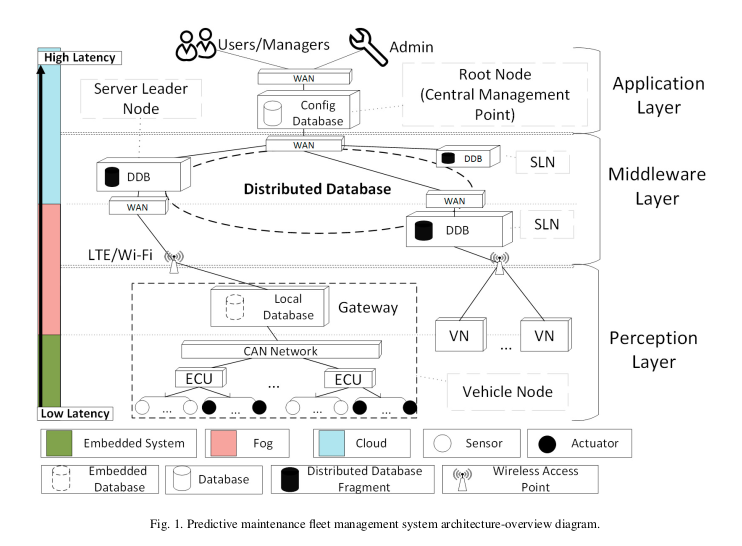
\includegraphics[scale=0.75]{architecture.png}
    \end{center}

     
    \section*{Protocols}
    %our understanding of what the authors have contributed or raised as comments regarding the topic.  
    \begin{enumerate}
        \item \textbf{MQTT}  - It stands for Message Queuing Telemetry Transport Protocol. This protocol is used for data transmission between IoT devices. It is lightweight, so it requires minimal resources. This protocol is scalable and can connect over unreliable cellular networks. It is secure and well-supported as several languages support its implementation 
        \item \textbf{SAE J1939} - It is the accepted industry standard for a vehicular network of off-highway machines in various application. It is a higher-layer protocol based on Controller Area Network (CAN) that facilitates serial data communications between microprocessor systems in heavy-duty vehicles. The messages exchanged between these units can be data such as vehicle road speed, torque control message from the transmission to the engine, oil temperature, etc.
       
    \end{enumerate}
 \section*{Agreement, Pitfalls and Fallacies}
    \begin{enumerate}
        \item Labeled datasets of vehicle faults are difficult to obtain considering it is financially not viable to deliberately damage the equipment in order to study faults. Faulty vehicles can be found and analysed and a system can be developed in order to keep track of faulty equipment for study purposes.
        \item Outlier scores are used to detect if the equipment is considered ‘normal’ or ‘anomaly’. It allows us to compare the degree of difference between two objects that have both been labeled ‘anomaly’. Other approaches such as counting objects in k-neighborhoods, kth nearest neighbor distances are not as helpful as this.
       			\item The sensor feature selection performed in COSMO is improved by using semi-supervised machine learning approach. I agree with this method as it will be able to capture the nuances that a human would be able to identify when working with the fleet on a day-to-day basis.
    \end{enumerate}
    \section*{Conclusion}
    The existing system of IoT-based maintenance of fleet management can be optimized by improving the sensor selection process. A proposed method to do so is ICOSMO, which takes a semi-supervised machine learning approach. Three layers are used in the novel architecture for fleet management- perception layer, middleware layer and application layer. They work in tandem to perform the required tasks more efficiently than the five layers of existing IoT architecture.
    
%\end{multicols}
\end{document}

